%%%%%%%%%%%%%%%%%%%%%%%%%%%%%%%%%%%%%%%%%
% Wenneker Article
% LaTeX Template
% Version 2.0 (28/2/17)
%
% This template was downloaded from:
% http://www.LaTeXTemplates.com
%
% Authors:
% Vel (vel@LaTeXTemplates.com)
% Frits Wenneker
%
% License:
% CC BY-NC-SA 3.0 (http://creativecommons.org/licenses/by-nc-sa/3.0/)
%
%%%%%%%%%%%%%%%%%%%%%%%%%%%%%%%%%%%%%%%%%

%----------------------------------------------------------------------------------------
%	PACKAGES AND OTHER DOCUMENT CONFIGURATIONS
%----------------------------------------------------------------------------------------

\documentclass[10pt, a4paper, twocolumn]{article}

%%%%%%%%%%%%%%%%%%%%%%%%%%%%%%%%%%%%%%%%%
% Wenneker Article
% Structure Specification File
% Version 1.0 (28/2/17)
%
% This file originates from:
% http://www.LaTeXTemplates.com
%
% Authors:
% Frits Wenneker
% Vel (vel@LaTeXTemplates.com)
%
% License:
% CC BY-NC-SA 3.0 (http://creativecommons.org/licenses/by-nc-sa/3.0/)
%
%%%%%%%%%%%%%%%%%%%%%%%%%%%%%%%%%%%%%%%%%
%we were here!! :D FERMI 

%----------------------------------------------------------------------------------------
%	PACKAGES AND OTHER DOCUMENT CONFIGURATIONS
%----------------------------------------------------------------------------------------

\usepackage[english]{babel} % English language hyphenation

\usepackage{microtype} % Better typography

\usepackage{amsmath,amsfonts,amsthm} % Math packages for equations

\usepackage[svgnames]{xcolor} % Enabling colors by their 'svgnames'

\usepackage[hang, small, labelfont=bf, up, textfont=it, position=below, skip=5pt]{caption} % Custom captions under/above tables and figures
\setlength{\belowcaptionskip}{-10pt}

\usepackage{booktabs} % Horizontal rules in tables

\usepackage{lastpage} % Used to determine the number of pages in the document (for "Page X of Total")

\usepackage{graphicx} % Required for adding images

\usepackage{enumitem} % Required for customising lists
\setlist{noitemsep} % Remove spacing between bullet/numbered list elements

\usepackage{sectsty} % Enables custom section titles
\allsectionsfont{\usefont{OT1}{phv}{b}{n}} % Change the font of all section commands (Helvetica)

\usepackage[pdfborder={0 0 0},colorlinks=true,linkcolor={black},citecolor={black},urlcolor={blue!60!black}]{hyperref}

%----------------------------------------------------------------------------------------
%	MARGINS AND SPACING
%----------------------------------------------------------------------------------------

\usepackage{geometry} % Required for adjusting page dimensions

\geometry{
	top=1cm, % Top margin
	bottom=1.5cm, % Bottom margin
	left=2cm, % Left margin
	right=2cm, % Right margin
	includehead, % Include space for a header
	includefoot, % Include space for a footer
	%showframe, % Uncomment to show how the type block is set on the page
}

\setlength{\columnsep}{7mm} % Column separation width

%----------------------------------------------------------------------------------------
%	FONTS
%----------------------------------------------------------------------------------------

\usepackage[T1]{fontenc} % Output font encoding for international characters
\usepackage[utf8]{inputenc} % Required for inputting international characters

\usepackage{XCharter} % Use the XCharter font

%----------------------------------------------------------------------------------------
%	HEADERS AND FOOTERS
%----------------------------------------------------------------------------------------

\usepackage{fancyhdr} % Needed to define custom headers/footers
\pagestyle{fancy} % Enables the custom headers/footers

\renewcommand{\headrulewidth}{0.0pt} % No header rule
\renewcommand{\footrulewidth}{0.4pt} % Thin footer rule

\renewcommand{\sectionmark}[1]{\markboth{#1}{}} % Removes the section number from the header when \leftmark is used

%\nouppercase\leftmark % Add this to one of the lines below if you want a section title in the header/footer

% Headers
\lhead{} % Left header
\chead{\textit{\thetitle}} % Center header - currently printing the article title
\rhead{} % Right header

% Footers
\lfoot{} % Left footer
\cfoot{} % Center footer
\rfoot{\footnotesize Page \thepage\ of \pageref{LastPage}} % Right footer, "Page 1 of 2"

\fancypagestyle{firstpage}{ % Page style for the first page with the title
	\fancyhf{}
	\renewcommand{\footrulewidth}{0pt} % Suppress footer rule
}

%----------------------------------------------------------------------------------------
%	TITLE SECTION
%----------------------------------------------------------------------------------------

\newcommand{\authorstyle}[1]{{\large\usefont{OT1}{phv}{b}{n}\color{DarkRed}#1}} % Authors style (Helvetica)

\newcommand{\institution}[1]{{\footnotesize\usefont{OT1}{phv}{m}{sl}\color{Black}#1}} % Institutions style (Helvetica)

\usepackage{titling} % Allows custom title configuration

\newcommand{\HorRule}{\color{DarkGoldenrod}\rule{\linewidth}{1pt}} % Defines the gold horizontal rule around the title

\pretitle{
	\vspace{-30pt} % Move the entire title section up
	\HorRule\vspace{10pt} % Horizontal rule before the title
	\fontsize{32}{36}\usefont{OT1}{phv}{b}{n}\selectfont % Helvetica
	\color{DarkRed} % Text colour for the title and author(s)
}

\posttitle{\par\vskip 15pt} % Whitespace under the title

\preauthor{} % Anything that will appear before \author is printed

\postauthor{ % Anything that will appear after \author is printed
	\vspace{10pt} % Space before the rule
	\par\HorRule % Horizontal rule after the title
	\vspace{20pt} % Space after the title section
}

%----------------------------------------------------------------------------------------
%	ABSTRACT
%----------------------------------------------------------------------------------------

\usepackage{lettrine} % Package to accentuate the first letter of the text (lettrine)
\usepackage{fix-cm}	% Fixes the height of the lettrine

\newcommand{\initial}[1]{ % Defines the command and style for the lettrine
	\lettrine[lines=3,findent=4pt,nindent=0pt]{% Lettrine takes up 3 lines, the text to the right of it is indented 4pt and further indenting of lines 2+ is stopped
		\color{DarkGoldenrod}% Lettrine colour
		{#1}% The letter
	}{}%
}

\usepackage{xstring} % Required for string manipulation

\newcommand{\lettrineabstract}[1]{
	\StrLeft{#1}{1}[\firstletter] % Capture the first letter of the abstract for the lettrine
	\initial{\firstletter}\textbf{\StrGobbleLeft{#1}{1}} % Print the abstract with the first letter as a lettrine and the rest in bold
}
 % Specifies the document structure and loads requires packages

%----------------------------------------------------------------------------------------
%	ARTICLE INFORMATION
%----------------------------------------------------------------------------------------

\title{My favorite physicist} % The article title

\author{
	\authorstyle{Group for Lasers and Plasmas\textsuperscript{$\ast,\dagger,\ddagger$}} % Authors
	\newline\newline % Space before institutions
	\textsuperscript{$\ast$}\institution{Institute for Plasmas and Nuclear Fusion}\\
	\textsuperscript{$\dagger$}\institution{Instituto Superior Técnico, Lisboa}\\
	\textsuperscript{$\ddagger$}\institution{\url{http://epp.ist.utl.pt/}}
}


\date{May 5, 2017}
%----------------------------------------------------------------------------------------


\begin{document}

\maketitle % Print the title

\thispagestyle{firstpage} % Apply the page style for the first page (no headers and footers)

%----------------------------------------------------------------------------------------
%	ABSTRACT
%----------------------------------------------------------------------------------------

\lettrineabstract{This is a small example of a showcase for a session on git/github. The main idea is to use some resources available only and add a section of one famous physicist. You can even use pictures of equations or something you associate with this person. It does not matter for now. Just use some reference if you are copying something. Everyone likes to be acknowledged.}

%----------------------------------------------------------------------------------------
%	ARTICLE CONTENTS
%----------------------------------------------------------------------------------------
\input{content/instruction.tex}

\input{content/albert_einstein.tex}
\section*{Ludwing Boltzmann\protect\footnote{\url{https://en.wikipedia.org/wiki/Ludwig_Boltzmann}}}

\begin{figure}[ht]
  \centering
  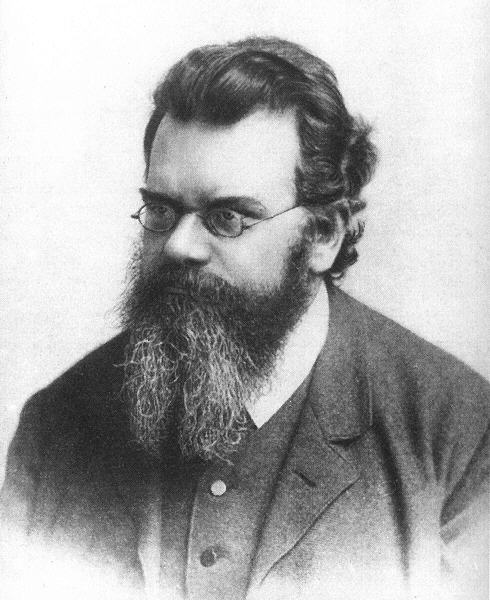
\includegraphics[width=0.8\linewidth]{content/figures/Boltzmann_figure.jpg}
  \caption{Albert Einstein in 1921\protect\footnotemark}
\end{figure}
\footnotetext{\url{https://upload.wikimedia.org/wikipedia/commons/a/ad/Boltzmann2.jpg}}

Boltzmann was born in Vienna, the capital of the Austrian Empire. His father, Ludwig Georg Boltzmann, was a revenue official. His grandfather, who had moved to Vienna from Berlin, was a clock manufacturer, and Boltzmann's mother, Katharina Pauernfeind, was originally from Salzburg. He received his primary education from a private tutor at the home of his parents. Boltzmann attended high school in Linz, Upper Austria. When Boltzmann was 15, his father died.

Boltzmann studied physics at the University of Vienna, starting in 1863. Among his teachers were Josef Loschmidt, Joseph Stefan, Andreas von Ettingshausen and Jozef Petzval. Boltzmann received his PhD degree in 1866 working under the supervision of Stefan; his dissertation was on kinetic theory of gases. In 1867 he became a Privatdozent (lecturer). After obtaining his doctorate degree, Boltzmann worked two more years as Stefan's assistant. It was Stefan who introduced Boltzmann to Maxwell's work.

In 1869 at age 25, thanks to a letter of recommendation written by Stefan,[2] he was appointed full Professor of Mathematical Physics at the University of Graz in the province of Styria. In 1869 he spent several months in Heidelberg working with Robert Bunsen and Leo Königsberger and then in 1871 he was with Gustav Kirchhoff and Hermann von Helmholtz in Berlin. In 1873 Boltzmann joined the University of Vienna as Professor of Mathematics and there he stayed until 1876.

In 1872, long before women were admitted to Austrian universities, he met Henriette von Aigentler, an aspiring teacher of mathematics and physics in Graz. She was refused permission to audit lectures unofficially. Boltzmann advised her to appeal, which she did, successfully. On July 17, 1876 Ludwig Boltzmann married Henriette; they had three daughters and two sons. Boltzmann went back to Graz to take up the chair of Experimental Physics. Among his students in Graz were Svante Arrhenius and Walther Nernst.[3][4] He spent 14 happy years in Graz and it was there that he developed his statistical concept of nature.

Boltzmann was appointed to the Chair of Theoretical Physics at the University of Munich in Bavaria, Germany in 1890. In 1893, Boltzmann succeeded his teacher Joseph Stefan as Professor of Theoretical Physics at the University of Vienna.

Boltzmann spent a great deal of effort in his final years defending his theories. He did not get along with some of his colleagues in Vienna, particularly Ernst Mach, who became a professor of philosophy and history of sciences in 1895. That same year Georg Helm and Wilhelm Ostwald presented their position on Energetics at a meeting in Lübeck. They saw energy, and not matter, as the chief component of the universe. Boltzmann's position carried the day among other physicists who supported his atomic theories in the debate.[5] In 1900, Boltzmann went to the University of Leipzig, on the invitation of Wilhelm Ostwald.[6] After the retirement of Mach due to bad health, Boltzmann returned to Vienna in 1902.[7] In 1903 he founded the Austrian Mathematical Society together with Gustav von Escherich and Emil Müller. His students included Karl Przibram, Paul Ehrenfest and Lise Meitner.

In Vienna, Boltzmann taught physics and also lectured on philosophy. Boltzmann's lectures on natural philosophy were very popular and received considerable attention. His first lecture was an enormous success. Even though the largest lecture hall had been chosen for it, the people stood all the way down the staircase. Because of the great successes of Boltzmann's philosophical lectures, the Emperor invited him for a reception at the Palace.

On September 5, 1906, while on a summer vacation in Duino, near Trieste, Boltzmann hanged himself.[8][9] He is buried in the Viennese Zentralfriedhof; his tombstone bears the inscription of the entropy formula:
\begin{equation}
	S=k\cdot \log W\,
\end{equation}


\end{document}
